\section{Introduction}

Flooding is one of the most significant natural disasters in the United States (US) affecting both the loss of life and property. 
In 2017 and 2019, river and flash flooding combined represented the leading cause of death among all natural disasters and in 2018 they were only second to deaths from heat wave \cite{national_weather_service_2020,national_weather_service_2019,national_weather_service_2018}. 
More than an average of 104 deaths per year are attributed to flood events from the 10 year period ending in 2019 \cite{us_department_of_commerce_2020}. 
Within that 10 year window, the most common activity victims were partaking in was driving when compared to other common activities leading to death \cite{us_department_of_commerce_2020}.
With respect to property damages, river and flash flooding have contributed to 60.7, 1.6, and 3.7 billion non-inflation adjusted US dollars in the annual periods of 2017 to 2019, respectively \cite{national_weather_service_2020,national_weather_service_2019,national_weather_service_2018}. 
The large spike in damages for 2017 can be attributed to the Hurricane Harvey event that primarily affected Texas in August. 
Unencouragingly, the trends related to flood damages and fatalities have been steadily increasing over recent decades. \cite{mallakpour2015changing,downton2005reanalysis,kunkel1999temporal,pielke2000precipitation,corringham2019effect}. 
Some are expecting that the hydrologic cycle will intensify which will lead to more extreme precipitation in some areas along with a greater risk of flooding \cite{tabari2020climate,milly2002increasing,wing2018estimates}. 
Increasing trends in frequency and risk are not uniform across spatial regions with work by \citeA{slater2016recent} indicating that trends are increasing across the US Midwest/Great Lakes region while decreasing in coastal Southeast, Southwest and California.


Operational flood forecasting systems are primary tools in developing accurate forecasts for public awareness prior to life or property damaging events occur. 
One of these operational systems is the Advanced Hydrologic Prediction System (AHPS) maintained by National Oceanic Atmospheric Administration (NOAA) National Weather Service (NWS) with approximately 3,781 forecast points across the US at typically short forecast horizons of 24 or 72 hours \cite{mcenery2005noaa}.
AHPS provides forecasting services in the form of ensemble streamflows at 3,781 forecast points illustrated in Figure \ref{fig:all_ahps_points} and flood inundation maps (FIM) at 188 of those forecast points shown in Figure \ref{fig:fim_ahps_points}.
AHPS implements a series of advances including model calibration techniques \cite{zhang2003hydrologic,hogue2003multi,duan2003global,gupta2003advances,parada2003multi}, distributed modeling approaches \cite{reed2004overall,koren2004hydrology,duan2002results}, ensemble forecasting \cite{day1985extended,seo2000simulation,mullusky2002simplified,herr2002simplified}, enhanced data analysis procedures \cite{mcenery2005noaa}, flood-forecasting inundation maps \cite{cajina2002fldview}, hydraulic routing models \cite{fread1973technique,cajina2002fldview}, and multisensor precipitation techniques \cite{breidenbach1999accounting,kondragunta2001outlier,seo2002real,bonnin1996noaa}.
Despite the AHPS advances in operational flood forecasting, its limitations are the lack of spatial coverage and short forecast time horizons.
Approximately, there is only one forecast point every 1,455 km of river and one forecast point with FIM every 29,261 km.

\begin{figure}[h!]
\centering
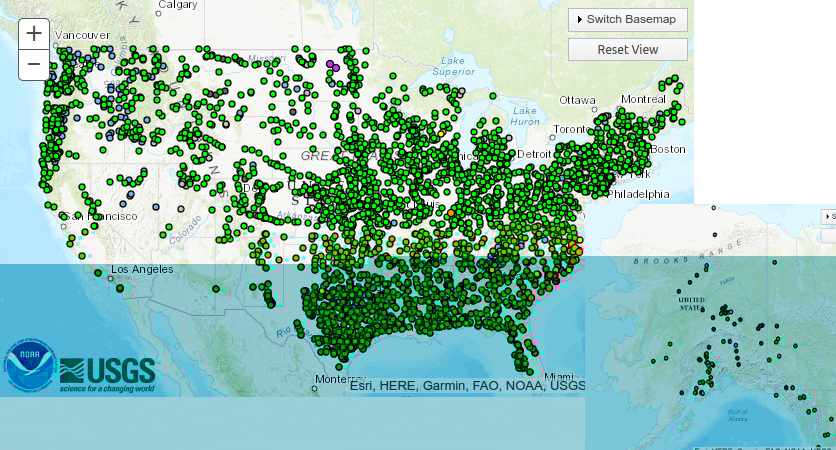
\includegraphics[scale=2.0]{figs/ahps_all_forecast_points.jpg}
\caption{All 3,781 forecast points in United States' Advanced Hydrologic Prediction System for lower 48 states and Alaska. No forecast points in Hawaii or territories. From: water.weather.gov/ahps}
\label{fig:all_ahps_points}
\end{figure}

\begin{figure}[h!]
\centering
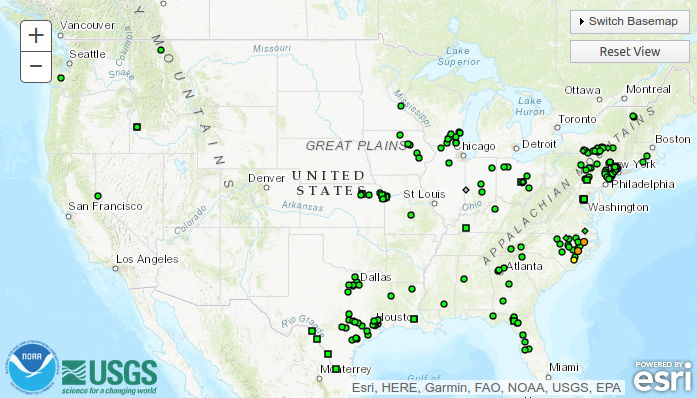
\includegraphics[scale=2.0]{figs/ahps_fim_forecast_points_conus.jpg}
\caption{All 188 forecast points in United States' Advanced Hydrologic Prediction System with flood inundation mapping capabilities. One forecast point near Juneau, Alaska not shown. No forecast points in Hawaii or remaining territories. From: water.weather.gov/ahps}
\label{fig:fim_ahps_points}
\end{figure}

Additional work is required to fill-in the gaps that the AHPS leaves in terms of spatial and temporal coverage.
To broaden the forecasting domain, the Office of Water Prediction (OWP) at the National Water Center (NWC) in Tuscaloosa, Alabama commissioned the development of the National Water Model (NWM) which is an instance of the Weather Research and Forecast Hydrologic Model (WRF-Hydro) \cite{gochis2018wrf,cosgrove2019evolution}. 
The NWM forecasts river discharges at more than 2.7 million forecast points at a variety of time horizons including some medium (10 day) and long (30 day) range forecast horizons.
The NWM enhances the spatial and temporal domain of the current AHPS capabilities at the 13 River Forecast Centers (RFC) in areas known as `hydro-blind' and is not meant to be a replacement. 
It's simply an additional model to be used in the forecasting and early warning decision making.
Furthermore, the NWM as of V1.2 has implemented not only assimilation of real-time United States Geological Survey (USGS) stage discharges but also assimilation of flow forecasts from the AHPS forecast points which are in turn routed downstream and updated whenever a new point is reached. This configuration of the NWM is known as `Replace and Route' or `RnR' and is used to enhance the forecasting skill of the NWM with the best available regional-scale data.


The National Hydrography Dataset Plus (NHDPlus) version 2.1 is the basis for the hydrofabric in the NWM due to its comprehensive use with the hydrologic communities' stakeholders \cite{mckay2012nhdplus}. 
The term hydrofabric is used within the NWM jargon to describe the subset of hydrography comprised of geospatial datasets required for hydrologic modeling including but not limited to stream networks, catchments, channel properties, and elevation data. 
The routing methods used within the NWM for its stream network is Muskingam-Cunge (MC) routing to reduce computational requirements of a continental scale model \cite{bedient2008hydrology,ponce1994variable,gochis2018wrf}.
Muskinham-Cunge routing scheme has been demonstrated by \citeA{cunge1969subject} to be equivalent to the convective-diffusive wave method without consideration to wave dampening.
As a result of high computational costs and large spatial domains, the need for high-resolution FIM at 10m or better requires additional post-processing from the principal output of the NWM which is forecast river discharges at the reach scale. The Height Above Nearest Drainage (HAND) terrain model is one such technique that can be used, along with synthetic rating curves (SRC), to convert riverine discharges to stages to inundation extents.

HAND normalizes topography along the nearest drainage path and its been demonstrated to be a good proxy and indicator of a series of important environmental conditions including soil environments, landscape classes, soil gravitational potentials, geomorphologies, soil moisture, and ground water dynamics \cite{renno2008hand,nobre2011height}. 
\citeA{nobre2016hand} showed evidence for utilizing the drainage normalizing HAND dataset as a proxy for flood potential to make static flood inundation maps from known stages. 
\citeA{zheng2018river} developed methodolgy for determing stage-discharge relationships known as synthetic rating curves (SRC) by sampling reach-averaged parameters from HAND datasets and inputting into the Manning's equation \cite{gauckler1867etudes,manning1890flow}.
This collection of methods, coupling HAND with SRCs, has been experimented and compared to other sources of FIM including engineering scale models, in-situ observation, and remote sensing based observation with solid results in large spatial scale applications \cite{godbout2019error,johnson2019integrated,garousi2019terrain,nobre2016hand,afshari2018comparison,zheng2018geoflood,teng2015rapid,teng2017flood,zhang2018comparative}.
Many of those assesing HAND's efficacy for producing FIM have noted opportunities for improvement. 
\citeA{godbout2019error} found how reach length and slope are important parameters for maximizing mapping skill with the moderate values performing best. 
The colinearity of reach length and slope led \citeA{godbout2019error} to propose that reaches of extreme lengths performed worse because of the extreme slope values, a parameter directly represented in Manning's equation. 
Issues with the reach-average approaches have been documented in \citeA{tuozzolo2019impact} where large within reach variance of the roughness Manning's n coefficient have been observed.
These works motivate splitting junction to junction reaches into smaller and equidistant segments for better averaging behaviour and SRC representation. 
Furthermore, \citeA{garousi2019terrain} noted improvements to mapping efficacy by conditioning monotonically decreasing thalweg elevations, adjusting the Manning's n roughness coefficient, and using higher resolution (3m) DEM's derived from light detection and ranging (Lidar).
Use of higher resolution DEMs in that study was motivated by previous work with Lidar DEMs and least-cost thalweg derivations \cite{zheng2018geoflood}.
Further work by \citeA{johnson2019integrated} noted the general under-prediction of HAND and suggested tuning the Manning's n parameter to better align SRC's with observations. 
Additionally, the sensitivity to low topographic relief and channel slope have been observed \cite{johnson2019integrated,godbout2019error}. 
Catchment boundary issues are noted where the interconnection of catchments are not properly accounted for \cite{zhang2018comparative,mcgehee2016modified}.
The HAND method and its associated advances require advanced computational algorithms and software to compute a FIM hydrofabric required for producing continental-scale FIM (CFIM).


Thanks to the availability of high-performance computing (HPC) and large scale high-resolution digital elevation models (DEM) such as the National Elevation Dataset (NED) at the 10m scale, HAND has been implemented into software for large-scale, continental computation. 
HAND was initially implemented into operational software by the National Flood Interoperability Experiment (NFIE) to generate FIM hydrofabric (will be used interchangebly with the datasets produced by HAND) rapidly on a high-performance computer (HPC) \cite{maidment2017conceptual,liu2016cybergis}. 
NFIE used open source dependencies including the Terrain Analysis Using Digital Elevation Models (TauDEM) \cite{tarboton2005terrain} and the Geospatial Data Abstraction Library (GDAL) \cite{warmerdam2008geospatial} to compute HAND for the Continental United States (CONUS) at 331 Hydrologic Unit Code (HUC) 6 processing units in 1.34 CPU years.
By allocating 31 nodes at 20 cores per for a total of 620 available cores to the overall operation, it enabled the production to finish up in 36 hours consuming 3.2TB of peak memory and 5TB of total disk space.
Originally, NFIE utilized the National Hydrography Dataset (NHD) Plus Medium Resolution (MR) to etch or burn flowlines prior to further conditioning but more recent work has advanced this to the more current NHDPlus High Resolution (HR) \cite{liu2020height}. 
The original NFIE dataset was employed by the NWC to produce forecast FIM from the NWM for use within its network of RFC's for additional guidance in hydro-blind regions and tagged as OWP's FIM version 1.0.
Further work by \citeA{djokic2019arc}, implemented a series of improvements to HAND inluding equi-distant reaches, updates to use with NHDPlusHR hydrography, and AGREE-DEM reconditioning \cite{hellweger1997agree} into an ESRI Arc-Hydro workflow with use in ArcGIS and tagged as OWP FIM v2.0. 
More notably the software added the ability to derive drainage potentials on a per mainstem basis as originally conceptualized by \cite{mcgehee2016modified}.
Mainstem is generally used here as defined in \citeA{blodgett2020mainstems} but only available in mainstems downstream of forecast AHPS points within the workflow introduced by \citeA{djokic2019arc}.
Overall, the software package is estimated to run CONUS at the full-resolution in 0.55 CPU years in a desktop setting.


To continue to innovate and implement the most advanced developments in FIM, the need arose to implement a more advanced software package with higher standards for specifications.

\begin{enumerate}
\item Use easily accesible, open-source dependencies to promote free-use, open-access, and community development and research.
\item Excellent single-core computational and memory performance with favorable, time and space complexities.
\item Ability to parallelize across multiple cores and nodes within HPC or cloud compute environments.
\item Preprocessing functionality within package pipeline to acquire and process input artificats.
\item Rapid inundation mapping capabilities to go from FIM hydrofabric datasets to forecast FIMs from NWM.
\item Automated testing functionality to ensure modifications enhance forecast skill when compared to external sources
\end{enumerate} 
